\section{Expressions}


\subsection{Syntax}


\begin{frame}{Introduction}
  Let's start with a very simple language.  
\end{frame}



\begin{frame}
  \frametitle{Language \lggeE}
    \[
  \begin{array}{llclll}
    \TYPES & \tau & \Coloneqq & \enum{}  & \enum{} & \text{numbers}
    \\
           &&& \estr{} & \estr{} & \text{strings}
    \\
    \\  \pause
    % 
    \EXPS & e & \Coloneqq  & \var{x} & \var{x} & \text{variable}
    \\
           &&& \enum{n} & n & \text{numeral}
    \\
           &&& \estr{s} & \litstr{s} & \text{literal}
    \\
           &&& \eplus{e_1}{e_2} & e_1 {+} e_2 & \text{addition}
    \\
           &&& \etimes{e_1}{e_2} & e_1 {*} e_2 & \text{multiplication}
    \\
           &&& \ecat{e_1}{e_2} & e_1 \concat e_2 & \text{concatenate}
    \\
           &&& \elen{e} & \lvert e \rvert & \text{length}
    \\
           &&& \elet{e_1}{x}{e_2} & \clet{e_1}{x}{e_2} & \text{definition}
  \end{array}
  \]



%%% Local Variables:
%%% mode: latex
%%% TeX-master: "main"
%%% End:

\end{frame}



% \note{A very simple language}


\begin{frame}
  \frametitle{The limits of syntax}
  \label{fr:syntax-e}
  Do all syntactically correct terms make sense?
  % 
  \pause
  
  \bigskip

  Examples:
  \begin{itemize}[<+->]
  \item $\eplus{\enum{3}}{\enum{4}}$
  \item $\elet{4}{x}{\eplus{\var{x}}{15}}$
  \item $\ecat{\enum{42}}{\estr{hello}}$
  \item $\elet{4}{x}{\eplus{\var{y}}{15}}$
  \end{itemize}



\end{frame}



\subsection{Typing system}

\begin{frame}
  \frametitle{Judgements}

  We will use judgements of the form:
  % 
  {\Huge
    \[
    {\tyjudge{\Gamma}{e}{\tau} }
    \]
  }
  which means ``$e$ has type $\tau$ under the hypotheses in $\Gamma$''.
  % 
  \pause
  % 
  \begin{itemize}
  \item $\Gamma$ is a \emph{context} which either empty (written $\varnothing$) or of the form:
    $\var{x}_1 : \tau_1, \ldots, \var{x}_n : \tau_n$ where
    $\forall i\neq j \qst \var{x}_i \neq \var{x}_j$.
    % 
  \item $e$ is an expression in $\lggeE$, e.g., $e = \enum{n}$,
    $e = \eplus{e_1}{e_2}$, etc.
    % 
  \item $\tau$ is a type in $\lggeE$, i.e., $\tau = \enum{}$ or
    $\tau = \estr{}$.
  \end{itemize}
  % 
\end{frame}


\note{

  \begin{itemize}
  \item   We write
    % 
    $\dom{\Gamma}$ for the \emph{domain} of $\Gamma$, i.e., if
    $\Gamma = \var{x}_1 : \tau_1, \ldots, \var{x}_n : \tau_n$, then
    $\dom{\Gamma} = \{ \var{x}_1  , \ldots, \var{x}_n \}$.
    % 
    % 
    % 
  \item We take the convention that when we write ``$\Gamma, \var{x} : \tau$'',
    we implicitly assume that $\var{x} \notin\dom{\Gamma}$.
  \end{itemize}




}


\begin{frame}
  \frametitle{Statics}

  The type system of $\lggeE$ is inductively defined by the following rules:
  
  \[
  \tyrule
  {\etyrulename{var}}
  {\,}
  {\tyjudge{\Gamma_1, \var{x}: \tau, \Gamma_2}{\var{x}}{\tau} }
  \]

  \pause
  \[
  \tyrule
  {\etyrulename{str}}
  {\,}
  {\tyjudge{\Gamma}{\estr{s}}{\estr{}}}
  \qquad\qquad\qquad
  \tyrule
  {\etyrulename{num}}
  {\,}
  {\tyjudge{\Gamma}{\enum{n}}{\enum{}}}
  % \end{array}
  \]
  

  \pause 
  \[
  \tyrule
  {\etyrulename{plus}}
  {
    \tyjudge{\Gamma}{e_1}{\enum{}}
    \and
    \tyjudge{\Gamma}{e_2}{\enum{}}
  }
  {\tyjudge{\Gamma}{\eplus{e_1}{e_2}}{\enum{}}}
  \]

  \pause 
  \[
  \tyrule
  {\etyrulename{times}}
  {
    \tyjudge{\Gamma}{e_1}{\enum{}}
    \and
    \tyjudge{\Gamma}{e_2}{\enum{}}
  }
  {\tyjudge{\Gamma}{\etimes{e_1}{e_2}}{\enum{}}}
  % 
  \]
\end{frame}


\begin{frame}
  \frametitle{Statics}
  \[
  \tyrule
  {\etyrulename{cat}}
  {
    \tyjudge{\Gamma}{e_1}{\estr{}}
    \and
    \tyjudge{\Gamma}{e_2}{\estr{}}
  }
  {\tyjudge{\Gamma}{\ecat{e_1}{e_2}}{\estr{}}}
  \]

  \bigskip
  \pause
  

  \[
  \tyrule
  {\etyrulename{len}}
  {
    \tyjudge{\Gamma}{e}{\estr{}}
  }
  {\tyjudge{\Gamma}{\elen{e}}{\enum{}}}
  \]

  \bigskip
  \pause

  \[
  \tyrule
  {\etyrulename{let}}
  {
    \tyjudge{\Gamma}{e_1}{\tau_1}
    \and
    \tyjudge{\Gamma, \var{x} : \tau_1 }{e_2}{\tau}
  }
  {\tyjudge{\Gamma}{\elet{e_1}{x}{e_2}}{\tau}}
  \]
\end{frame}

\begin{frame}
  \frametitle{Well-typed}
  \label{fr:types-e}

  Term $e$ is \emph{well-typed} iff there is $\tau$ such that
  $\tyjudge{\varnothing}{e}{\tau}$ is derivable according the static
  rules of the language.

  \pause
  \bigskip

  Are these $\lggeE$ phrases well-typed?
  \begin{itemize}[<+->]
  \item $\ecat
    {\ecat
      {\estr{\text{hello}}}   
      {\estr{\text{world}}}
    }
    {\estr{\text{!}}}$
  \item $\etimes
    {\elen{\estr{\text{hello}}}}
    {\eplus{\enum{1}}{\elen{\estr{\text{world}}}}}$
    % 
  \item $\elet{\estr{\text{mystring}}}{x}{\etimes{\elen{\var{x}}}{\enum{0}}}$
    % 
  \item $\elet
    {\estr{\text{anotherstring}}}
    {y}
    {\eplus{\var{y}}{\etimes{\enum{1}}{\enum{2}}}}$
    % 
  \item $\elet
    {\ecat{\estr{\text{anotherstring}}}{\var{y}}}
    {y}
    {\var{y}}$
  \end{itemize}
\end{frame}


\begin{frame}
  \frametitle{Type systems: summary}

  \begin{itemize}
  \item Type systems restrict the set of ``allowed'' programs.
    % 
  \item Type systems are defined through a set of (inductively
    defined) typing rules.
    % 
  \item Type systems do not say anything about the \emph{meaning} of
    programs.
    % 
  \item Type systems enforce \emph{static} properties of programs.
  \end{itemize}
\end{frame}

% \begin{frame}
%   \frametitle{Housekeeping}
%   \begin{itemize}[<+->]
%   \item Recording of lecture \#2: I'll upload last year's
%     lecture.
%   \item Temperature in KLT5
%   \end{itemize}
%   \pause
%   \includegraphics[scale=0.7]{roomtemp.png}
% \end{frame}

\begin{comment}
\begin{frame}
  \frametitle{Last week}
  {\Huge 
    \[
    \tyjudge{\Gamma}{e}{\tau}
    \]
  }
  \pause 
  \begin{itemize}
  \item $\Gamma$ is an \emph{environment} that keeps track of declared
    variables and their types. 
    % 
  \item At the start of a type checking derivation, no variable is
    declared, hence $\Gamma = \varnothing$ (i.e., $\Gamma$ is empty).
    % 
  \item In language $\lggeE$:
    \begin{itemize}
    \item only rule {\etyrulename{let}} adds elements in $\Gamma$ 
    \item only rule {\etyrulename{var}} queries $\Gamma$.
    \end{itemize}
  \item The letter $\Gamma$ is a \emph{meta-variable}, it should never
    appear in a type derivation (just like $e_i$ and $\tau$).
  \end{itemize}
\end{frame}

\begin{frame}
  \frametitle{Last week}
  {\small
    \[
    \tyrule{{let}}
    {
      \tyrule{{num}}
      {\,}
      {
        \tyjudge{\varnothing}
        {\enum{42}}
        {\enum{}}
      }
      \\
      % 
      \tyrule{{plus}}
      {
        \tyrule{{var}}
        {\,}
        {
          \tyjudge{\var{z} : \enum{}}
          {\var{z}}
          {\enum{}}
        }
        \\
        % 
        \tyrule{{num}}
        {\,}
        {
          \tyjudge{\var{z} : \enum{}}
          {\enum{1}}
          {\enum{}}
        }
      }
      { 
        \tyjudge{\var{z} : \enum{}}
        {\eplus{\var{z}}{\enum{1}}}
        {\enum{}}
      }
    }
    {
      \tyjudge{\varnothing}
      {\elet{\enum{42}}{z}{\eplus{\var{z}}{\enum{1}}}}
      {\enum{}}
    }
    \]
  }

  \bigskip
  
  \begin{tabular}{l}
    NB: \;
    ${\elet{\enum{42}}{z}{\eplus{\var{z}}{\enum{1}}}}$ 
    \\
    \qquad   \qquad    stands for: \;  $ {\clet{\enum{42}}{z}{\eplus{\var{z}}{\enum{1}}}}$
  \end{tabular}
\end{frame}
\end{comment}

\begin{frame}
  \frametitle{Abstract Binding Tree}
  \begin{itemize}[<+->]
  \item \textbf{Concrete syntax} is concerned with how phrases are
    entered and displayed on a computer, e.g., $\clet{e_1}{x}{e_2}$.
    % 
  \item \textbf{Abstract syntax} is concerned with the \emph{structure} of
    phrases, specifically how they are composed from other phrases,
    $\eplus{e_1}{\etimes{e_2}{e_3}}$.
    % 
  \item At the ``abstract level'' a phrase is a tree (data structure),
    called an \emph{abstract syntax tree}, whose nodes are operators
    that combine several phrases to form another phrase.
    \begin{center}
      E.g., see the \texttt{Term} data type in
      \href{https://github.com/rgrig/plad/blob/master/code/Lambda.hs}{Radu's
        $\lambda$-calculus interpreter}. 
    \end{center}
    % 
  \item \textbf{Abstract binding trees} (ABT) enrich abstract syntax
    trees with the concepts of \emph{binding} and \emph{scope}, e.g., $\elet{e_1}{x}{e_2}$. 
    \begin{itemize}
    \item Binding: introduction of a new variable/parameter/name.
    \item Scope: the sub-tree where an identifier may be used.
    \end{itemize}
  \end{itemize}
\end{frame}


\begin{frame}
  \frametitle{Binders and Closed / Open terms}
  \begin{itemize}[<+->]
  \item Construct $\elet{e_1}{x}{e_2}$ is a \emph{binder}, it binds $\var{x}$ in $e_2$.
    \[
    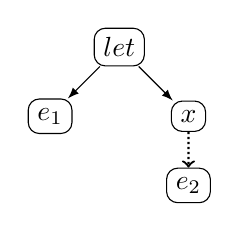
\begin{tikzpicture}[
      edge from parent/.style={draw,-latex},
      sibling distance=5em,
      level distance=2.5em,
      every node/.style = {shape=rectangle, rounded corners,
        draw, align=center,
        top color=white}]]
      \node {$\kw{let}$}
      child { node {$e_1$} }
      child { node {$\var{x}$}
        child { node {$e_2$} edge from parent[thick, densely dotted,->]
        }
      };
    \end{tikzpicture}
    \]
  \item \emph{Bound variable:} a variable under a binder, e.g.,
    $\elet {\estr{\text{hello}}} {x} {\ecat{\var
        x}{\estr{\text{world}}}}$
    % 
  \item A variable that is not bound is \emph{free}. A term with
    free-variables is \emph{open}, e.g., in
    $\elet{\estr{\text{hello}}}{x}{\ecat{\var x}{{{\var{y}}}}}$,
    $\var{y}$ is \emph{free}.
    % 
  \item A consequence of $e$ being well-typed is that it is
    \emph{closed}, i.e., $e$ has no free variable.
    % 
  \end{itemize}
\end{frame}



\subsection{Semantics}


\begin{frame}
  \frametitle{Semantics}
  The semantics of a programming language define what a program
  \emph{means}, i.e., how a program \emph{evaluates}.

  \bigskip

  The semantics of a programming language define ``dynamic''
  properties of the language, i.e., how programs ``move''.
  
\end{frame}

\begin{frame}
  \frametitle{Dynamics}
  \label{fr:value-e}

  The judgement ``$\valjudge{e}$'' states that $e$ is a value (i.e.,
  cannot be reduced further, it is the final result of a computation).
  % 
  % 
  % 
  It is inductively defined by the following two rules:
  \[
  \semrule{}
  {\,}
  {\valjudge{\enum{n}}}
  \qquad \qquad  \qquad
  \semrule{}
  {\,}
  {\valjudge{\estr{s}}}
  \]

  \bigskip
  \pause

  Are these values (i.e., does  $\valjudge{e}$ hold)?
  \begin{itemize}[<+->]
  \item $\estr{\text{hello}}$
  \item $\elet
    {\estr{\text{anotherstring}}}
    {y}
    {\eplus{y}{\etimes{\enum{1}}{\enum{2}}}}$
  \end{itemize}
\end{frame}



\begin{frame}
  \frametitle{Dynamics}
  
  Now, we define the actual semantics of language $\lggeE$, it is
  defined via judgement of the form: $\jtrans{e}{e'}$.
  % 
  
  \bigskip

  The transition judgement $\jtrans{e}{e'}$ between states is
  inductively defined by the following rules:

  \pause

  \[
  \semrule
  {\esemrulename{plval}}
  {n_1 + n_2 = n}
  {\jtrans{\eplus{\enum{n_1}}{\enum{n_2}}}{\enum{n}}}
  \]

  \pause

  \[
  \semrule
  {\esemrulename{pll}}
  {\jtrans{e_1}{e'_1}}
  {\jtrans{\eplus{e_1}{e_2}}{\eplus{e'_1}{e_2}}}
  \]
  
  \pause

  \[
  \semrule
  {\esemrulename{plr}}
  { \valjudge{e_1}
    \and
    \jtrans{e_2}{e'_2}}
  {\jtrans{\eplus{e_1}{e_2}}{\eplus{e_1}{e'_2}}}
  \]
  
\end{frame}


\begin{frame}
  \frametitle{Dynamics}

  \[
  \semrule
  {\esemrulename{tmval}}
  {n_1 \times n_2 = n}
  {\jtrans{\etimes{\enum{n_1}}{\enum{n_2}}}{\enum{n}}}
  \]

  \pause

  \[
  \semrule
  {\esemrulename{tml}}
  {\jtrans{e_1}{e'_1}}
  {\jtrans{\etimes{e_1}{e_2}}{\etimes{e'_1}{e_2}}}
  \]
  
  \pause

  \[
  \semrule
  {\esemrulename{tmr}}
  { \valjudge{e_1}
    \and
    \jtrans{e_2}{e'_2}}
  {\jtrans{\etimes{e_1}{e_2}}{\etimes{e_1}{e'_2}}}
  \]
  
\end{frame}


% \note{Exercise: give are the rules for $\etimes{e_1}{e_2}$?}


\begin{frame}
  \frametitle{Dynamics}
  \[
  \semrule
  {\esemrulename{catval}}
  {s_1 \concat s_2 = s}
  {\jtrans{\ecat{\estr{s_1}}{\estr{s_2}}}{\estr{s}}}
  \]


  \pause

  \[
  \semrule
  {\esemrulename{catl}}
  { \jtrans{e_1}{e'_1}}
  {\jtrans{\ecat{e_1}{e_2}}{\ecat{e'_1}{e_2}}}
  \]
  
  \pause

  \[
  \semrule
  {\esemrulename{catr}}
  {\valjudge{e_1}
    \and
    \jtrans{e_2}{e'_2}}
  {\jtrans{\ecat{e_1}{e_2}}{\ecat{e_1}{e'_2}}}
  \]
  

\end{frame}


\begin{frame}
  \frametitle{Dynamics}
  \begin{itemize}[<+->]
  \item  Call-by-name:
    \[
    \semrule
    {\esemrulename{letn}}
    {\,}
    {
      \jtrans{\elet{e_1}{x}{e_2}}{\subs{e_2}{e_1}{x}}}
    \]
  \item   Call-by-value:

    \[
    \semrule
    {\esemrulename{letm}}
    {\jtrans{e_1}{e'_1}}
    {
      \jtrans{\elet{e_1}{x}{e_2}}{\elet{e'_1}{x}{e_2}}}
    \]
    \[
    \semrule
    {\esemrulename{letv}}
    {\valjudge{e_1}}
    {
      \jtrans{\elet{e_1}{x}{e_2}}{\subs{e_2}{e_1}{x}}}
    \]
  \end{itemize}

  \bigskip 

  \pause

  Is call-by-name semantics equivalent to laziness
  (like the default behaviour in Haskell)?
  % 
  What kind of strategy does OCaml use?

\end{frame}

\begin{frame}
  \frametitle{Evaluation strategies}
  \begin{itemize}[<+->]
  \item \emph{Call-by-value:} arguments are evaluated to values
    \emph{before} being substituted in for variables. Main advantage:
    program's behavior (easy to determine when an expression is
    evaluated) and performance (each expression is evaluated at most
    once). Main disadvantage: evaluate everything, even if not needed.
    % 
  \item \emph{Call-by-name:} arguments are substituted without being
    computed. Main advantage: expressions whose value is never needed
    are not evaluated (evaluate as late as possible). Main
    disadvantage: requires a lot of memory.
    % 
  \item \emph{Call-by-need:} arguments are not evaluated until their
    values are needed, but once they are evaluated, the value is
    \emph{recorded} so that it can be reused. Main advantage:
    expressions are evaluated at most once.
    % 
    Good trade-off between CBV and CBN but harder to implement
    correctly and efficiently.
  \end{itemize}
\end{frame}

\begin{frame}
  \frametitle{Call-by-name vs.\ call-by-value}
  % 
  \label{fr:srategies-e}
  % 
  What are the advantages/disadvantages of call-by-name vs.\ call-by-value?


  \bigskip

  Consider the following programs:
  \begin{itemize}
  \item $\elet{\etimes{1852}{2017}}{x}{\eplus{\var{x}}{\var{x}}}$
  \item $\elet{\etimes{1852}{2017}}{x}{\eplus{\var{1}}{\var{x}}}$
  \item $\elet{\etimes{1852}{2017}}{x}{\eplus{\var{1}}{\var{13}}}$
  \end{itemize}
\end{frame}

\begin{frame}
  \frametitle{Examples}
  \label{fr:evaluate-e}

  Evaluate these $\lggeE$ phrases:
  \begin{itemize}
  \item $\ecat
    {\ecat
      {\estr{\text{hello}}}   
      {\estr{\text{world}}}
    }
    {\estr{\text{!}}}$
  \item $\etimes
    {\elen{\estr{\text{hello}}}}
    {\eplus{\enum{1}}{\elen{\estr{\text{world}}}}}$
    % 
  \item $\elet{\estr{\text{mystring}}}{x}{\etimes{\elen{\var{x}}}{\enum{0}}}$
    % 
  \item $\elet
    {\estr{\text{anotherstring}}}
    {\var{y}}
    {\eplus{\var{y}}{\etimes{\enum{1}}{\enum{2}}}}$
  \end{itemize}
\end{frame}

\begin{frame}
  \frametitle{Feedback from Week 19}
  \begin{itemize}
  \item Missed lectures: hard to catch up.
  \item How to break down expressions?
  \item Difficulty understanding binders (let)
  \item When to apply plr or pll, and why is there separate rules?
  \item Whether we should write ``$\valjudge{e}$'' judgements explicitly
  \item Syntax of substitutions
  \item Terminology rule names, gamma ($\Gamma$), tau ($\tau$)
  \item Full definitions of all languages will be on Moodle
  \end{itemize}
\end{frame}

\begin{frame}
  \frametitle{Recap}
  Judgements covered so far:
  
  \bigskip
  
  \begin{itemize}
    \setlength\itemsep{1.5em}
  \item \emph{Type system:}
    $\tyjudge{\var{x_1} : \tau_1, \ldots, \var{x_k}:\tau_k}{e}{\tau}$
    means that, assuming that variable $\var{x_i}$ has type $\tau_i$
    ($\forall 1 \leq i \leq k$), term $e$ has type $\tau$.
    % 
  \item \emph{Semantics (1):} $\valjudge{e}$ means that term $e$ is a \emph{value} (it
    cannot be evaluated further).
    % 
  \item \emph{Semantics (2):} $\jtrans{e}{e'}$ means that term $e$
    evaluate to term $e'$ (in one step).
  \end{itemize}
\end{frame}



%%% Local Variables:
%%% mode: latex
%%% TeX-master: "main"
%%% End:


\begin{frame}
  \label{fr:ite-e}
  \frametitle{Exercise}
  Add the following construct to language $\lggeE$:
  \[
  \site{e}{e_1}{e_2}
  \qquad\qquad \text{i.e.,} \quad
  \csite{e}{e_1}{e_2}
  \]
  
  \bigskip
  
  Think of what you will need to add wrt.\ syntax, types, and
  semantics.
\end{frame}




\subsection{Type safety}


\begin{frame}
  \frametitle{Type safety}
  \begin{itemize}
  \item We want \emph{type safe} programming languages
    % 
  \item i.e., certain kinds of mismatches cannot happen at runtime,
    e.g., we would like to avoid computation like: \texttt{``one'' == 123}.
    % 
  \item \emph{Type safety} expresses the \emph{coherence} between
    statics (types) and dynamics (semantics).
    % 
  \item A consequence of type safety is that evaluation cannot get stuck.
  \end{itemize}
\end{frame} 


\begin{frame}
  \frametitle{Type safety}\label{fr:ty-safety}

  Hereafter, we often write $\tyjudge{\,}{e}{\tau}$ for
  $\tyjudge{\varnothing}{e}{\tau}$.

  \bigskip 

  \pause

  \begin{theorem}[Type safety]
    \begin{enumerate}[<+->]
    \item If $\tyjudge{}{e}{\tau}$ and $\jtrans{e}{e'}$, then $\tyjudge{}{e'}{\tau}$.
    \item If $\tyjudge{}{e}{\tau}$, then either $\valjudge{e}$, or there exists $e'$ such that $\jtrans{e}{e'}$.
    \end{enumerate}
  \end{theorem}


  The first part of the theorem is often referred to as \emph{type
    preservation}, while the second part is referred to as
  \emph{progress}.
\end{frame}



\begin{frame}
  \frametitle{Runtime errors}

  Suppose we extend $\lggeE$ with a division operator:
  $\ediv{e_1}{e_2}$.
  

  \begin{itemize}
  \item  A natural typing rule is:
    \pause 
    \[
    \tyrule
    {\etyrulename{div}}
    {
      \tyjudge{\Gamma}{e_1}{\enum{}}
      \and
      \tyjudge{\Gamma}{e_2}{\enum{}}
    }
    {\tyjudge{\Gamma}{\ediv{e_1}{e_2}}{\enum{}}}
    % 
    \]

  \item    Main semantics rule: 
    \pause
    % 
    % 
    \[
    \semrule
    {\esemrulename{dval}}
    {n_1 \div n_2 = n}
    {\jtrans{\ediv{\enum{n_1}}{\enum{n_2}}}{\enum{n}}}
    \]

    
  \end{itemize}


  \pause 

  \bigskip

  \emph{Problem:} the expression $\ediv{\enum{3}}{\enum{0}}$ is
  \emph{well-typed}, yet ``\emph{stuck}''!
  % 
  
  % 
\end{frame}
\begin{frame}
  \frametitle{Runtime errors}

  \emph{Two possible solutions:}


  \bigskip

  \begin{itemize}[<+->]
  \item \emph{Enhanced the type-system}, so that no well-typed program
    may divide by zero.
    % 
  \item Add \emph{dynamic checks}, so that division-by-zero signals an error
    (of evaluation).
  \end{itemize}


  \pause
  
  \bigskip
  
  The first approach may rule out too many ``good'' programs.
  % 
  In general, we cannot predict \emph{statically} whether an
  expression will be non-zero when evaluated.
  

  \bigskip
  
  Hence, the second approach is generally preferred.
  % 
\end{frame}



\begin{frame}
  \frametitle{Checked vs. Unchecked errors}
  We need to distinguish between \emph{checked} and \emph{unchecked errors}.
  \bigskip
  \begin{description}
    \setlength\itemsep{2em}
    % 
  \item[Unchecked error:] ruled out by the type system. No run-time
    checking performed because the type system rules out the
    possibility of such errors arising.
    % 
  \item[Checked error:] not ruled out by the type system, hence
    run-time check \emph{must} occur, e.g., a zero divisor.
  \end{description}
\end{frame}



\begin{frame}
  \frametitle{Dealing with run-time error}
  % 
  \[
  \semrule
  {\esemrulename{dval}}
  {n_1 / n_2 = n \and n_2 > 0}
  {\jtrans{\ediv{\enum{n_1}}{\enum{n_2}}}{\enum{n}}}
  \]


  \pause
  
  \[
  \semrule
  {\esemrulename{dval}}
  {\,}
  {\jtrans{\ediv{\enum{n_1}}{\enum{0}}}{\eerror}}
  \]

  \pause

  \[
  \semrule
  {\esemrulename{dl}}
  {\jtrans{e_1}{e'_1}}
  {\jtrans{\ediv{e_1}{e_2}}{\ediv{e'_1}{e_2}}}
  \]

  \pause

  \[
  \semrule
  {\esemrulename{dr}}
  { \valjudge{e_1}
    \and
    \jtrans{e_2}{e'_2}}
  {\jtrans{\ediv{e_1}{e_2}}{\ediv{e_1}{e'_2}}}
  \]
  

  \pause
  \bigskip

  Note $\eerror$ is a new term in language $\lggeE$.
  \pause
  % 
  \[
    \tyrule
    {\etyrulename{err}}
    {
      \,
    }
    {\tyjudge{\Gamma}{\eerror}{\tau}}
      % 
    \]
  
\end{frame}


\begin{frame}
  \frametitle{Dealing with run-time error}
  
  How do we preserve \emph{type safety} with run-time errors?

  \bigskip
  \pause
  

  \emph{Idea:} use expression $\eerror$ (i.e., a \emph{checked} error)
  and define a judgement $\errjudge{e}$ stating that $e$ incurs a
  run-time checked error.
  % 
  % \[
  % \anorule
  % {\valjudge{e_1}}
  % {\errjudge{\ediv{e_1}{\enum{0}}}}
  % \quad
  % \anorule
  % {\errjudge{e_1}}
  % {\errjudge{\ediv{e_1}{e_2}}}
  % \quad
  % \anorule
  % {\valjudge{e_1}
  % \and \errjudge{e_2}}
  % {\errjudge{\ediv{e_1}{e_2}}}
  % \]

  \[
  \anorule{\,}{\errjudge{\eerror}}
  \]

  \begin{theorem}[Progress with error]
    % 
    If $\tyjudge{}{e}{\tau}$, then either $\errjudge{e}$, $\valjudge{e}$, or there
    exists $e'$ such that $\jtrans{e}{e'}$.
    % 
  \end{theorem}
\end{frame}


\begin{frame}
  \frametitle{Discussion}

  Do we need to update the \textbf{type preservation} statement?

  \pause
  \bigskip
  
  Can you think of other \textbf{examples} of checked / unchecked errors?
\end{frame}


%%% Local Variables:
%%% mode: latex
%%% TeX-master: "main"
%%% End:
